\chapter{Dealing with low density chains}
\label{low-density}


\section{Introduction}

\subsection{Recap: stability windows}
\label{low-density:recap-stability-window}

Blocks are validated against ledger states; each block is validated against the
ledger state as it was after applying the previous block. This means that when
we validate block $B$ in the example below, we use the ledger state after
applying block $A$; for block $C$, we use the ledger state after applying block
$B$:
%
\begin{center}
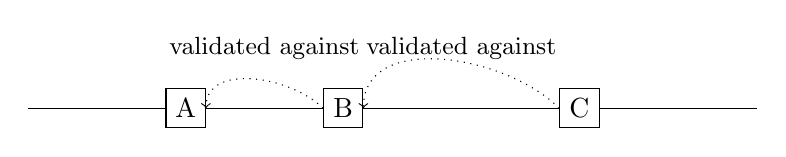
\begin{tikzpicture}
  [block/.style={rectangle,draw=black,minimum size=5mm}
  ,baseline=0pt]
\node at (0,0) (A) [block] {A};
\node at (2,0) (B) [block] {B};
\node at (5,0) (C) [block] {C};
\draw (-2,0)   -- (A.west);
\draw (A.east) -- (B.west) node[pos=0.5,above=5mm]{\small validated against};
\draw (B.east) -- (C.west) node[pos=0.5,above=5mm]{\small validated against};
\draw (C.east) -- ++(2,0);
%
\draw [->, dotted] (B.west) to [out=135,in=90] (A.east);
\draw [->, dotted] (C.west) to [out=135,in=90] (B.east);
\end{tikzpicture}
\qquad
\begin{minipage}{0.25\textwidth}
\emph{Horizontal axis represents time (in slots)}
\end{minipage}
\end{center}
%
In the chain sync client (\cref{chainsyncclient}) we are however not validating
blocks, but block \emph{headers}. In order to validate a header, we only
need part of the ledger state: the ledger \emph{view}; but, despite the fact
that we only need part of the ledger state, we cannot \emph{update} the ledger
view using only headers: we still need the full block (this is similar to what
we described in \cref{hfc:failed:forecasting}). This means that if we have block
$A$, but only block \emph{headers} $B$ and $C$, we have a problem:
%
\begin{center}
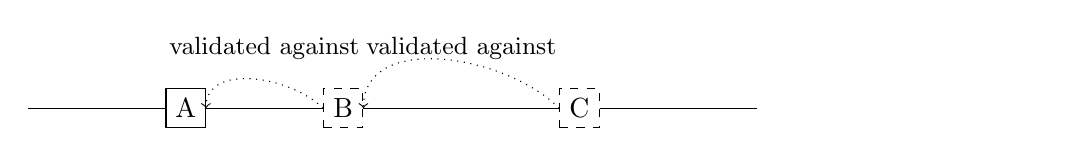
\begin{tikzpicture}
  [block/.style={rectangle,draw=black,minimum size=5mm}]
\path (-2,0) -- (11,0); % adjust bounding box
\node at (0,0) (A) [block] {A};
\node at (2,0) (B) [block, dashed] {B};
\node at (5,0) (C) [block, dashed] {C};
\draw (-2,0)   -- (A.west);
\draw (A.east) -- (B.west) node[pos=0.5,above=5mm]{\small validated against};
\draw (B.east) -- (C.west) node[pos=0.5,above=5mm]{\small validated against};
\draw (C.east) -- ++(2,0);
%
\draw [->, dotted] (B.west) to [out=135,in=90] (A.east);
\draw [->, dotted] (C.west) to [out=135,in=90] (B.east);
\end{tikzpicture}
\end{center}
%
Validating header $B$ is unproblematic, since we have the ledger state available
after applying block $A$. However, since we don't have block $B$, we can't
compute the ledger state after block $B$ to validate header $C$. We are saved by
the fact that we can \emph{forecast} the ledger view  required to validate
header $B$ from the ledger state after $A$:
%
\begin{center}
\begin{tikzpicture}
  [block/.style={rectangle,draw=black,minimum size=5mm}]
\path (-2,0) -- (11,0); % adjust bounding box
\node at (0,0) (A) [block] {A};
\node at (2,0) (B) [block, dashed] {B};
\node at (5,0) (C) [block, dashed] {C};
\draw (-2,0)   -- (A.west);
\draw (A.east) -- (B.west) node[pos=0.55,below=5mm]{\small forecast};
\draw (B.east) -- (C.west);
\draw (C.east) -- ++(2,0);
%
\draw [->, dotted] (B.west) to [out=135,in=90] (A.east);
\draw [->, dotted] (C.west) to [out=135,in=90] (B.east);
%
\draw [->, dotted] (A.east) to [out=270,in=270] (B.east);
\end{tikzpicture}
\end{center}
%
We can do this because of a restriction on the ledger: blocks cannot affect
the ledger view until a \emph{stability window} has passed:
%
\begin{center}
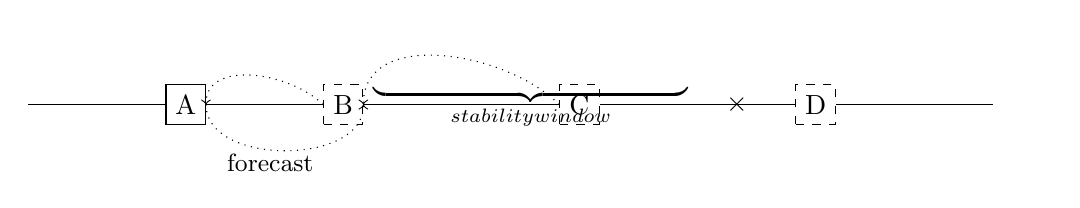
\begin{tikzpicture}
  [block/.style={rectangle,draw=black,minimum size=5mm}]
\path (-2,0) -- (11,0); % adjust bounding box
\node at (0,0) (A) [block] {A};
\node at (2,0) (B) [block, dashed] {B};
\node at (5,0) (C) [block, dashed] {C};
\node at (8,0) (D) [block, dashed] {D};
\draw (-2,0)   -- (A.west);
\draw (A.east) -- (B.west) node[pos=0.55,below=5mm]{\small forecast};
\draw (B.east) -- (C.west);
\draw (C.east) -- (D.west);
\draw (D.east) -- ++(2,0);
%
\draw [->, dotted] (B.west) to [out=135,in=90] (A.east);
\draw [->, dotted] (C.west) to [out=135,in=90] (B.east);
%
\draw [->, dotted] (A.east) to [out=270,in=270] (B.east);
\node at (B.east) [below=0.8, right] {$\underbrace{\hspace{4cm}}_\text{stability window}$};
\node at (7,0) {$\times$};
\end{tikzpicture}
\end{center}
%
We can use the ledger state after applying block $A$ (which we
have complete knowledge of) to validate any header up to the end of $B$'s
stability window: any changes that $A$ (or any block before $A$)
initiates we know about, and any changes that $B$ initiates cannot take effect
until that stability window ends. Therefore we can validate header $C$, but not
header $D$: block $B$ might have scheduled some changes to take effect at the
slot marked as $(\times)$ in the diagram, and we do not know what those effects
are.\footnote{It might be tempting to think that we can validate $D$ because if
we did have blocks $B$ and $C$, block $D$ would be evaluated against the ledger
state as it was after applying $C$, which is still within $B$'s stability
window. However, the slot number of $D$ (its location on the $x$-axis in the
diagram) matters, because changes are scheduled for slots.}

In the chain sync we do not currently take advantage of the knowledge of the
location of header $B$.\footnote{\label{footnote:anchor-after-first-header}We
should change this. By anchoring the stability window at the last known block,
we only have a guarantee that we can validate $k$ headers, but we should really
be able to validate $k + 1$ headers in order to get a chain that is longer than
our own (\cref{low-density:tension}). If we anchored the stability window after
the first unknown header, where it \emph{should} be anchored, we can validate
$k$ headers \emph{after} the first unknown header, and hence $k + 1$ in total.
Concretely, we would have to extend the \lstinline!LedgerSupportsProtocol! class
with a function that forecasts the ledger view given a \emph{ticked} ledger
state. Taking advantage of this would then just be a minor additional
complication in the chain sync client.}  This means we have to be conservative:
all we know is that there could be \emph{some} block in between $A$ and $C$ that
might schedule some changes that are relevant for validating header $C$. In this
case we therefore assume that the stability window extends from $A$ instead:
%
\begin{center}
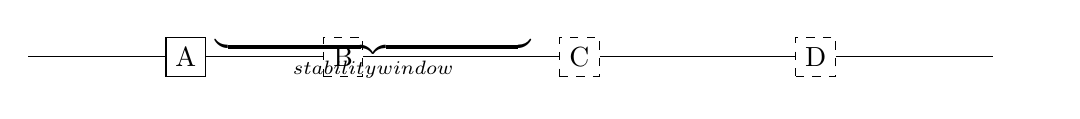
\begin{tikzpicture}
  [block/.style={rectangle,draw=black,minimum size=5mm}]
\path (-2,0) -- (11,0); % adjust bounding box
\node at (0,0) (A) [block] {A};
\node at (2,0) (B) [block, dashed] {B};
\node at (5,0) (C) [block, dashed] {C};
\node at (8,0) (D) [block, dashed] {D};
\draw (-2,0)   -- (A.west);
\draw (A.east) -- (B.west);
\draw (B.east) -- (C.west);
\draw (C.east) -- (D.west);
\draw (D.east) -- ++(2,0);
%
\node at (A.east) [below=0.8, right] {$\underbrace{\hspace{4cm}}_\text{stability window}$};
\end{tikzpicture}
\end{center}
%
In this example, that means we can validate $B$, but not $C$ (nor
$D$).\footnote{We could in principle shift this up by 1 slot: after all, the
very first next block after $A$ cannot be in the same slot as $A$. While EBBs
are an exception to that rule (\cref{ebbs}), we do not need to validate EBBs so
this is a rare example where EBBs do not cause a problem.}

\subsection{Tension with chain selection}
\label{low-density:tension}

Changes that affect the ledger view are scheduled for slots (often
for epoch boundaries, which happen at particular slots); it therefore makes
sense to define the stability window in terms of slots as well. This means that
the number of \emph{headers} we can validate within a given stability window
depends on the density of that chain; if the chain we considered at the end
of the previous section looks like this instead
%
\begin{center}
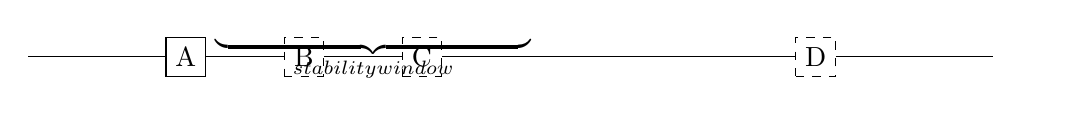
\begin{tikzpicture}
  [block/.style={rectangle,draw=black,minimum size=5mm}]
\path (-2,0) -- (11,0); % adjust bounding box
\node at (0,0) (A) [block] {A};
\node at (1.5,0) (B) [block, dashed] {B};
\node at (3,0) (C) [block, dashed] {C};
\node at (8,0) (D) [block, dashed] {D};
\draw (-2,0)   -- (A.west);
\draw (A.east) -- (B.west);
\draw (B.east) -- (C.west);
\draw (C.east) -- (D.west);
\draw (D.east) -- ++(2,0);
%
\node at (A.east) [below=0.8, right] {$\underbrace{\hspace{4cm}}_\text{stability window}$};
\end{tikzpicture}
\end{center}
%
we can validate headers $B$ and $C$ (but still not $D$).

There is a fundamental tension between the stability window defined in
\emph{slots}, and chain selection preferring  longer chains: chains that have
more \emph{blocks}. In order to be able to do a meaningful comparison between
our chain and the candidate chain, we must be able to verify enough of that
candidate chain that the length of that verified prefix exceeds the length of
our own chain. Since the maximum rollback we support is $k$
(\cref{consensus:overview:k}), that means we must be able to validate at least
$k + 1$ headers. The tension is resolved by a theoretical result that says that
within $3k/f$ slots we \emph{will} see more than $k$ blocks (more precisely, the
probability that we see fewer than $k$ blocks in $3k/f$ slots is negligibly
small; \cite{cryptoeprint:2017:573}). This therefore provides us with a suitable
choice for a stability window.

Unfortunately, while in theory there is no difference between theory and
practice, there is in practice. Currently, when all nodes in the system are
unable to produce blocks for an extended period of time, the system grinds to a
halt. Even if the underlying problem is resolved, nodes will refuse to create a
block if the distance between that block and the previous block exceeds the
stability; after all, if they did produce a block, other nodes would be unable
to validate it. The former is easily resolved, this is merely a check in the
block production code; resolving the second problem is the topic of this
chapter. As it turns out, we will need a different approach before and after
implementing the genesis chain selection rule (\cref{genesis}); we will discuss
these in sections~\ref{low-density:pre-genesis}
and~\ref{low-density:post-genesis}, respectively.

It would be preferable to avoid the tension altogether, and schedule
changes that affect the ledger view for particular \emph{blocks} instead
(and consequently, have epoch boundaries also happen at certain blocks). This
however requires backing from theoretical research; we will come back to this
in \cref{future:block-vs-slot}.

\subsection{Single-gap case}

It is tempting to think that when there is only a \emph{single} large gap
on the chain, there is no problem:
%
\begin{center}
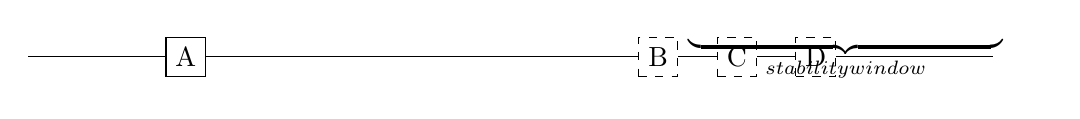
\begin{tikzpicture}
  [block/.style={rectangle,draw=black,minimum size=5mm}]
\path (-2,0) -- (11,0); % adjust bounding box
\node at (0,0) (A) [block] {A};
\node at (6,0) (B) [block, dashed] {B};
\node at (7,0) (C) [block, dashed] {C};
\node at (8,0) (D) [block, dashed] {D};
\draw (-2,0)   -- (A.west);
\draw (A.east) -- (B.west);
\draw (B.east) -- (C.west);
\draw (C.east) -- (D.west);
\draw (D.east) -- ++(2,0);
%
\node at (B.east) [below=0.8, right] {$\underbrace{\hspace{4cm}}_\text{stability window}$};
\end{tikzpicture}
\end{center}
%
Although there is a large gap (one that exceeds the stability window) between
$A$ and $B$, this should not matter: as we saw in
\cref{low-density:recap-stability-window}, it's not the stability window after
$A$ that matters, but the stability window after $B$. This seems to be a useful
special case: if a problem \emph{does} arise that prevents nodes from producing
blocks for an extended period of time, one might hope that this problem does not
immediately arise again after the nodes resume producing blocks.

As we saw, the consensus layer always conservatively anchors the stability
window at the last known block rather than the first header after the tip. We
could change this (and probably should; see
\cref{footnote:anchor-after-first-header}), but it turns out this does not
actually help very much for this particular problem. To see this, suppose there
is another node in the system which is currently on a fork that intersects with
this chain after some block $I$ before the gap:
%
\begin{center}
\begin{tikzpicture}
  [block/.style={rectangle,draw=black,minimum size=5mm}]
\node at (-2,-1) (I) [block] {I};
\node at (0,0) (A) [block, dashed] {A};
\node at (6,0) (B) [block, dashed] {B};
\node at (7,0) (C) [block, dashed] {C};
\node at (8,0) (D) [block, dashed] {D};
\draw (-4,-1)   -- (I.west);
\draw (I.east) -- (A.west);
\draw (A.east) -- (B.west);
\draw (B.east) -- (C.west);
\draw (C.east) -- (D.west);
\draw (D.east) -- ++(2,0);
%
\node at (A.east) [below=0.8, right] {$\underbrace{\hspace{4cm}}_\text{stability window}$};
%
\node at (0, -2) (A') [block] {A$'$};
\draw (I.east) -- (A'.west);
\end{tikzpicture}
\end{center}
%
The second node must execute a rollback to $I$ in order to be able to adopt
the new chain, but from \emph{its} perspective the first unknown block is $A$,
not $B$: hence the stability window \emph{must} be anchored at $A$, and the
node will be unable to bridge the gap.

\section{Pre-genesis}
\label{low-density:pre-genesis}

In this section we will consider how we might allow nodes to recover from a low
density chain, prior to the implementation of the genesis rule. An obvious
solution suggests itself: we could just  allow chain sync to download blocks
when it needs to validate a header which is beyond its forecast range.

Unfortunately, this opens us up to denial of service attacks: nothing is
stopping an attacker with even a small amount of stake from creating chains
with many large gaps on them, forcing us to download many blocks and compute
the corresponding ledger states. This is the very reason we don't download
blocks in the chain sync client in the first place
(\cref{nonfunctional:network:headerbody}).

We therefore need to limit \emph{when} we allow the chain sync client to
download blocks. It is difficult to come up with a rule that would allow us to
make \emph{local} (per peer) decisions, but we can impose a global rule

\begin{definition}[Side condition for downloading blocks in chain sync, pre-genesis]
\label{low-density:pre-genesis-jump-condition}
We only allow the chain sync client to download blocks when \emph{all} chain
sync clients are blocked because they received a header that is outside the
forecast range.
\end{definition}

This means that under normal circumstances, we will never download any blocks at
all, and so attackers cannot take advantage of this. We will download blocks
only when the system is stuck and there is a big gap on the chain, which is
precisely the problem that we are trying to solve. It does mean that an attacker
could make us do a bit more work in the narrow span of time when we are bridging
the gap, but that is no major concern. Note that unlike in the implementation of
the genesis rule (\cref{genesis}), we do not need to increase the number of
peers to connect to in order to make this decision: when we allow chain sync to
download blocks, we consider \emph{more} chains, not fewer.

A more serious worry is that an attacker might \emph{prevent} us from allowing
chain sync to download blocks by providing us with a chain that doesn't contain
any big gaps. This is however not a new concern. If the honest nodes in the
system are prevented from forging blocks due to some problem, this is a
dangerous state of affairs: if a malicious node does continue forging a chain at
this point, other nodes may well end up adopting this chain; after all, it is
longer than the honest chain (which has stalled). What's worse, they might adopt
more than $k$ blocks from that malicious chain, and so would be unable to roll
back to the honest chain once that starts to grow again. This is already true
even if we don't implement the change proposed in this section. A solution might
be to discard candidate chains if their density falls below a certain threshold;
this would stop nodes from adopting a bad chain even if the honest chain has
stalled, and also stops attackers from preventing us from allowing chain sync to
download blocks. Either way, the change proposed in this section does not make
this situation any worse.

\section{Post-genesis}
\label{low-density:post-genesis}

The situation changes a little once we implement the genesis chain selection
rule; in the following discussion we will assume that we will implement
Ouroboros Genesis following the recommendations from \cref{genesis}.

If no nodes are able to produce blocks for a period that exceeds the stability
window, then by definition\footnote{This will be true whether or not we look at
the immutable tip or the volatile tip to determine the switch-over point.} the
nodes will all be in conservative chain selection mode
(\cref{genesis:intro:conservative}). Recall from
\cref{genesis:insufficient-blocks} that when we encounter a node whose chain
terminates before the end of the look-ahead window, we disconnect from that
node:
%
\begin{center}
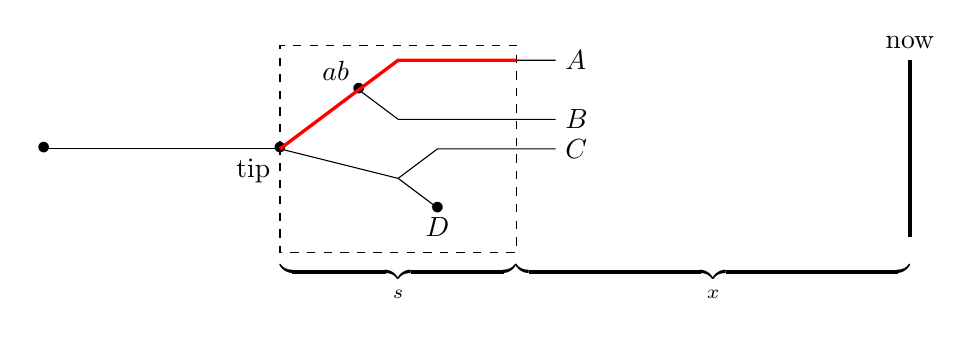
\begin{tikzpicture}[yscale=0.75]
\path (0, 0) coordinate (tip) node{$\bullet$} node[below left]{tip};
\draw (tip) -- ++(1.0,  1.0) coordinate (ab) node{$\bullet$} node[above left]{$ab$};
\draw (tip) -- ++(1.5, -0.5) coordinate (cd);
\draw (ab) -- ++(0.5,  0.5) -- ++(2.0, 0) node[right]{$A$};
\draw (ab) -- ++(0.5, -0.5) -- ++(2.0, 0) node[right]{$B$};
\draw (cd) -- ++(0.5,  0.5) -- ++(1.5, 0) node[right]{$C$};
\draw (cd) -- ++(0.5, -0.5) coordinate(D) node{$\bullet$} node[below]{$D$};

\draw [dashed]
     (tip)
  -- ++(0, 1.75)
  -- ++(3, 0)
  -- ++(0, -3.5)
  -- ++(-3, 0) node[pos=0.5, below]{$\underbrace{\hspace{3cm}}_s$}
  -- cycle;

\draw [red, very thick] (tip) -- (ab) -- ++(0.5,  0.5) -- ++(1.5, 0) ;
\draw (tip) + (-3,0) node{$\bullet$} -- (tip);

%
\draw [ultra thick] (8,-1.5) -- (8,1.5) node[above]{now};
\node at (5.5, -2.25) {$\underbrace{\hspace{5cm}}_x$};
\end{tikzpicture}
\end{center}
%
The justification for this rule is that if the tip of that candidate's chain is
before the end of the look-ahead window, that tip must be more than $x$ slots
away from the wallclock; moreover,  we picked $x$ to be large enough that we can
conclude that this means that the node itself is not up to date with the
network. We can therefore disconnect from the peer, at least temporarily.

But now consider what happens when no more blocks are being produced due to some
problem affecting all nodes. In this case, \emph{all} nodes have chains that
terminate within the look-ahead window:\footnote{ In fact, if we decide to
execute a roll-back when entering genesis mode, it is likely that all nodes
terminate near at the \emph{start} of the look-ahead window: after all, nodes
will anchor their look-ahead window at their immutable tip; that immutable tip
might not be the same for every node, depending on exactly how many blocks they
managed to adopt, but it will probably not differ by much.}
%
\begin{center}
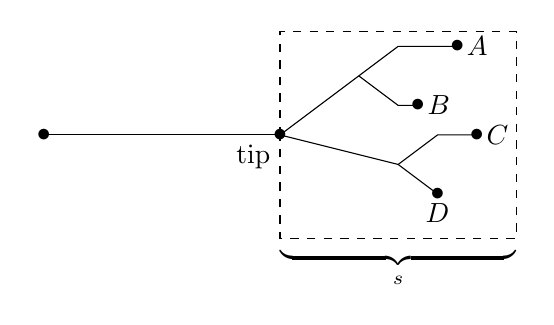
\begin{tikzpicture}[yscale=0.75]
\path (0, 0) coordinate (tip) node{$\bullet$} node[below left]{tip};
\draw (tip) -- ++(1.0,  1.0) coordinate (ab);
\draw (tip) -- ++(1.5, -0.5) coordinate (cd);
\draw (ab) -- ++(0.5,  0.5) -- ++(0.75, 0) node{$\bullet$} node[right]{$A$};
\draw (ab) -- ++(0.5, -0.5) -- ++(0.25, 0) node{$\bullet$} node[right]{$B$};
\draw (cd) -- ++(0.5,  0.5) -- ++(0.50, 0) node{$\bullet$} node[right]{$C$};
\draw (cd) -- ++(0.5, -0.5) coordinate(D) node{$\bullet$} node[below]{$D$};

\draw [dashed]
     (tip)
  -- ++(0, 1.75)
  -- ++(3, 0)
  -- ++(0, -3.5)
  -- ++(-3, 0) node[pos=0.5, below]{$\underbrace{\hspace{3cm}}_s$}
  -- cycle;

\draw (tip) + (-3,0) node{$\bullet$} -- (tip);
\end{tikzpicture}
\end{center}
%

If we just applied the rule as-is, we would disconnect from every upstream peer
and would have no way of making progress. We therefore make a small modification
to the rule:

\begin{definition}[Disconnect due to insufficient blocks]
We \emph{only} disconnect from an upstream peer if its chain terminates before
the end of the look-ahead window \emph{and} there are other chains that
\emph{do} fill the look-ahead window.
\end{definition}

The next problem is that once nodes do start producing again, we will end up
with a candidate that contains a larger-than-stability-window gap. The solution
here is the same as for the pre-genesis case (\cref{low-density:pre-genesis}):
we will allow chain sync to download blocks. As for the pre-genesis case, we
must be careful not to open ourselves up to DoS attacks, but the rule is
effectively the same (compare to \cref{low-density:pre-genesis-jump-condition}):

\begin{definition}[Side condition for downloading blocks in chain sync, post-genesis]
\label{low-density:post-genesis-jump-condition}
We only allow the chain sync client to download blocks in conservative mode, and
only when \emph{all} upstream chains contain a header that is outside the
forecast range.
\end{definition}

The final problem is that when nodes are in conservative mode, they do not
normally produce any blocks. After all, what would we do with such a block?
We could not adopt it, because by definition in conservative mode we only
adopt blocks that we are sure will never be rolled back, but we do not have
that certainty about a block we produce ourselves. Nonetheless in order to
get out of the impasse, we need a way to leave conservative mode and kick-start
the system again. We can do this as follows:

\begin{definition}[Kick-starting the chain in genesis mode]
When a node is running in conservative mode and notices that all its upstream
peers have chains that terminate before the end of the look-ahead, and it has
the right to produce a block for the current wallclock slot, it will do so,
forging a block on the current immutable tip.
\end{definition}

The immutable tip is the only block we can be sure about; it does not make much
sense to extend any of the other chains, as we have no good way of comparing
them (since they do not span $s$ slots, we have too few blocks to do a density
comparison). For the other nodes, this new block means a rollback, but a
rollback of at most $s$ slots, which will be less than $k$ blocks, so that
should not pose a problem. For the node that produced the new block, its chain
will now immediately have a tip near the wallclock, and so it will indeed leave
genesis mode.

% Note: this is an argument against looking at the % immutable tip (which anyway seems dangerous to me: the immutable tip may well fall in and out of that % $3k/f$ window), and anyway we don't need the previous argument that we can only fit so many gaps into % the distance between the tip and the wallclock to guard against attackers, because we'd not download % blocks whilst in speculative mode.

\section{Scope for abuse}

TODO. \todo{TODO} We can now cope with low density chains, but is the system
still secure in this case? Many assumptions from the Ouroboros papers are now
violated. A question for the researchers.
